\section{introduction}
\label{submission}

Unsupervised learning for deep reinforcement learning (DRL) is challenging
in the sense that agent should interact with the world and collect data to get a useful information
without explicit reward. In the pretraining step, agent gathers information from the environment
and learns representations of visited states, dynamics, and behaviors. When the downstream tasks are
given, the agent has to quickly adapt to them leveraging those representations. Recent works has shown that
skill discovery is a promising way to learn diverse behaviors which potentially help the agent achieve a goal
 \cite{salge2014empowerment, gregor2016variational, eysenbach2018diversity}.

\begin{figure}[ht]
    \vskip 0.2in
    \begin{center}
    % \centerline{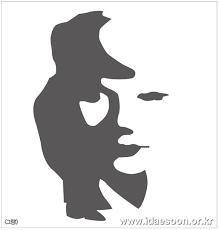
\includegraphics[width=\columnwidth]{Figures/perspective_different_pic.png}}
    \centerline{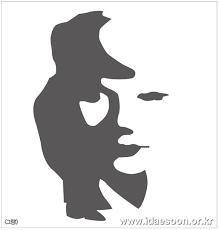
\includegraphics[width=0.5\columnwidth]{Figures/perspective_different_pic.png}}
    \caption{The picture looks different depending on the point of view}
    \label{perspective}
    \end{center}
    \vskip -0.2in
    \end{figure}
  

Although the agent could learn diverse skills, it is not obvious at a glance
how the agent manages them to solve a downstream task since the agent has to efficiently and effectively handle
multiple policies while the agent has just one policy to control in a typical reinforcement learning framework. Following the recent work \cite{laskin2021urlb} which evaluated a variety of unsupervised RL algorithms in locomotion environment, skill-based algorithms shows a poor performance compared to other algorithms.
Meanwhile, since the learned skills do not cover all the possible behaviors of agent practically,
agent is required to choose as appropriate skill for each moment or have an ability to combine several skills together.

One might simply use one of the skills best fitted for each task or sequentially 
perform a series of skills. However, these do not fully extract the potential which the learned skill has.
Instead, we explore the fine tuning method by focusing on how each skill views each state
and utilize them with weight.

Our main contribution is to emphasize the importance of fine tuning in skill discovery
by showing the finetuning method can affect the final score a lot for each task.
We also propose a simple but powerful finetune method utilizing every learned skill.